\documentclass{article}
\usepackage[T1]{fontenc}
\usepackage{circuitikz}
\begin{document}

\pgfcircversion

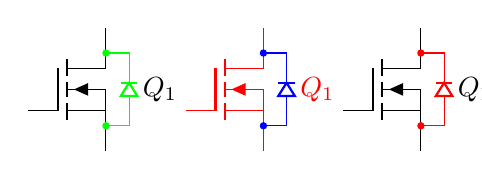
\begin{tikzpicture}[
    % define styles
    bodydiode color/.style={bodydiode,
    circuitikz/transistor bodydiode/color=#1},
    bodydiode red/.style={bodydiode color=red},
    ]
    % "manually"
    \draw (0,0) node (mosfet1) [nigfete,anchor=D,bodydiode,
        circuitikz/transistor bodydiode/color=green ] {$Q_1$};
    % with astyle with a parameter
    \draw (2,0) node (mosfet2) [nigfete, red, anchor=D, bodydiode color=blue] {$Q_1$};
    % with a fixed style
    \draw (4,0) node (mosfet3) [nigfete,anchor=D, bodydiode red] {$Q_1$};
\end{tikzpicture}
\end{document}